\subsection{Back-end module architecture}
This section shows how the Back-end\textsubscript{G} module of \textit{EmporioLambda} works. \\The Back-end\textsubscript{G} is based on the microservices/serverless pattern, where every function that manages an API request can be individually deployed and managed. Practically, the module is managed by the developers as a monolith, that can be divided in 3 layers:
\begin{itemize}
\item \textbf{Handler:} manages the API requests;
\item \textbf{Model:} manages the objects used by the module;
\item \textbf{Services:} manages the external services, like AWS and Stripe;
\end{itemize} 

The Front-end\textsubscript{G} module interacts with the Back-end one through API calls, exposed by AWS\textsubscript{G} API Gateway. This service sorts those requests to the \textbf{Handler} layer of the architecture, that consists of AWS\textsubscript{G} Lambda functions, divided by domains.\\
The function in charge of managing the request will call the \textbf{Services} layer to receive an interface to the main external services used.\\
If necessary, the function in question will use the \textbf{Model} layer to manage the objects it uses, like products or users.\\

The module can be summarized in the following scheme: 

\begin{figure}[H]
\centering
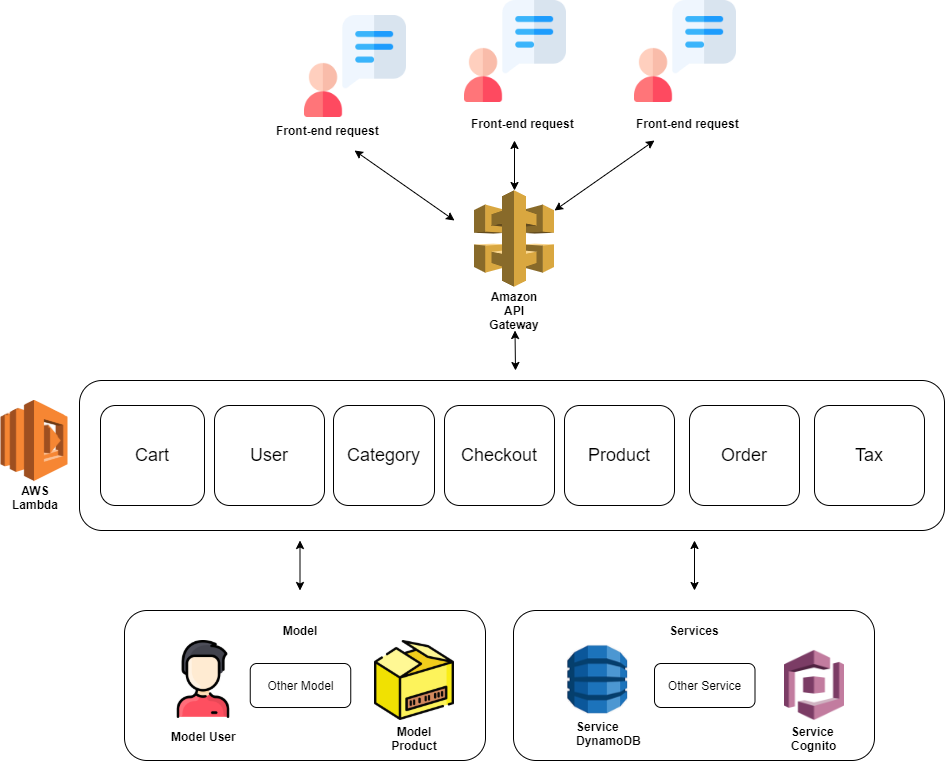
\includegraphics[scale=0.45]{res/Architettura/Backend/img/layerBack-end}\\
\caption{Back-end\textsubscript{G} module general scheme}
\end{figure}

The module can be also represented by the following package diagram:

\begin{figure}[H]
\centering
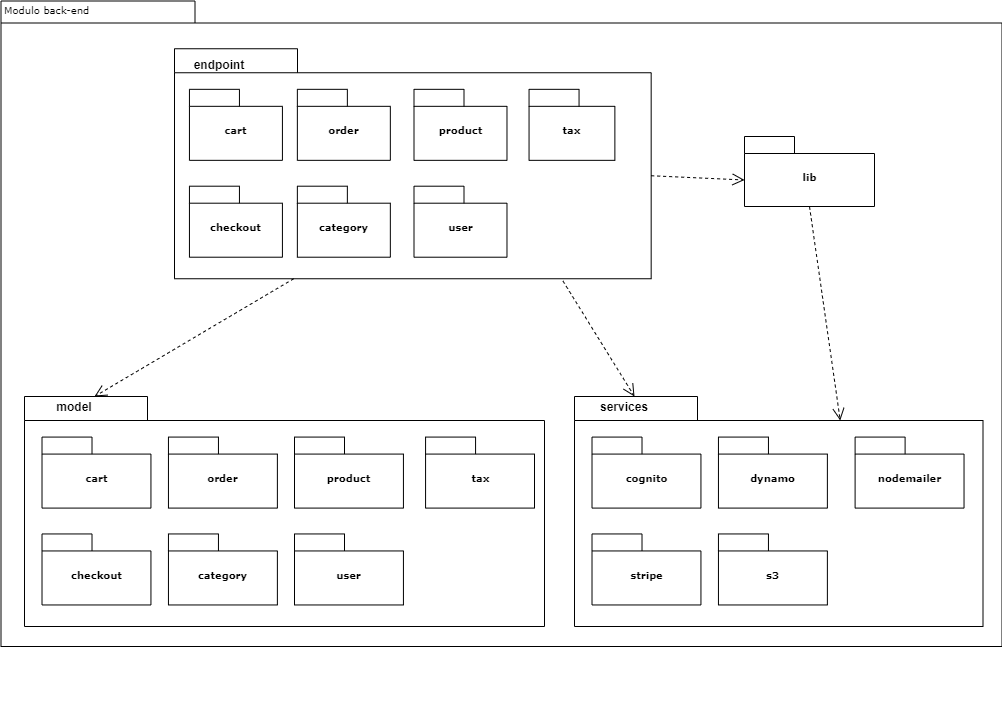
\includegraphics[scale=0.45]{res/Architettura/Backend/img/package-back-end}\\
\caption{Back-end\textsubscript{G} package diagram}
\end{figure}

\begin{itemize}
\item \textbf{endpoint}: it's the \textbf{Handler} layer described previously;
\item \textbf{services}: it's the \textbf{Services} layer described previously;
\item \textbf{model}: it's the \textbf{Model} layer described previously;
\item \textbf{lib}: contains support functions used by the endpoint package. One example is the management of the API response.
\end{itemize}

All of these packages can be found on the \textit{src} folder, divided in folders named by their package name.

\subsubsection{Model}
The \textbf{Model} layer represents the objects used by the \textbf{Handler} layer. \\
In the following class diagram we show every class used in the layer.

\begin{figure}[H]
\centering
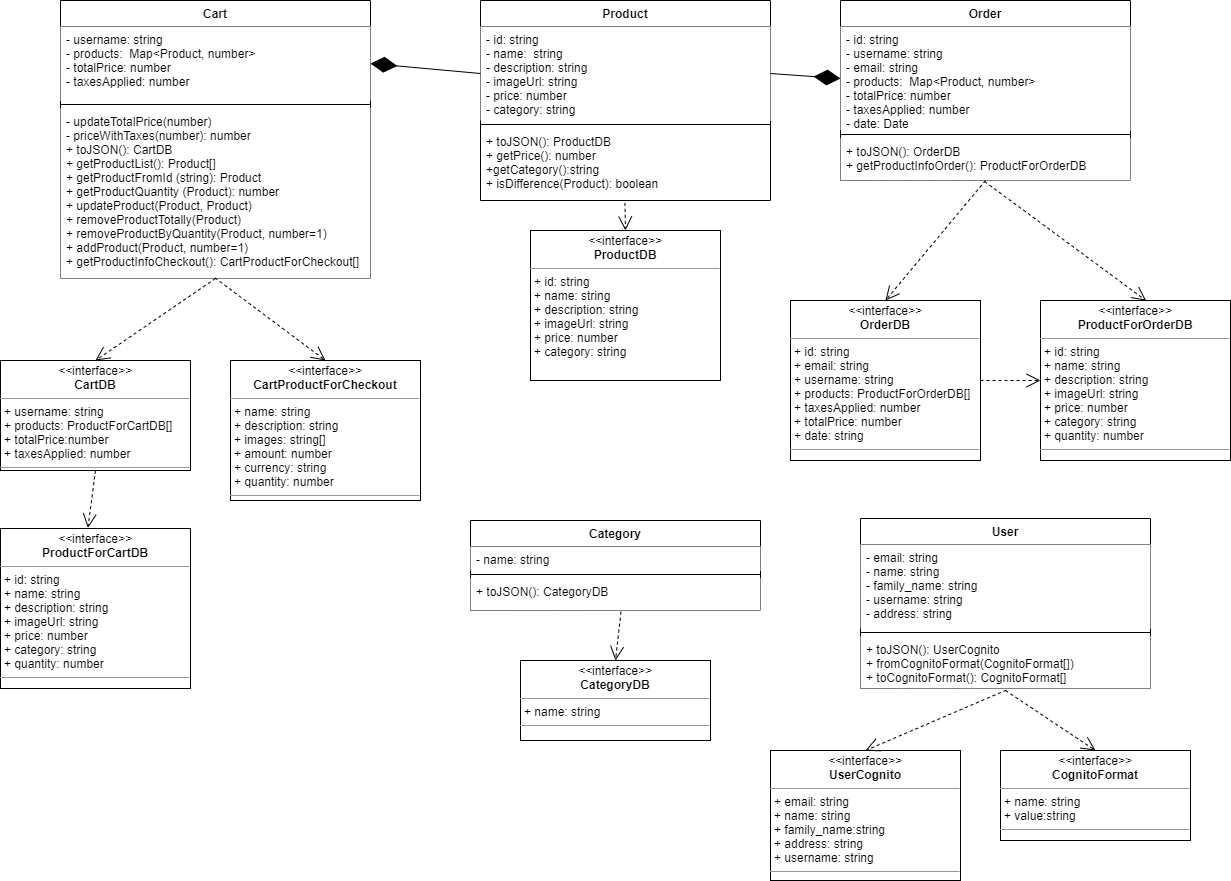
\includegraphics[scale=0.40]{res/Architettura/Backend/img/diagrammaClassiBack-end}\\
\caption{Back-end\textsubscript{G} Model layer class diagram}
\end{figure}



\subsubsection{Services}
The \textbf{Services} layer contains the functions used to create an interface for external services, like AWS\textsubscript{G} DynamoDB or Stripe\textsubscript{G}.\\
In the following class diagram we show every typescript\textsubscript{G} module used. We will represent every module as a class, since it contains public functions and it's used as a cached singleton, thanks to the typescript definition.

\begin{figure}[H]
\centering

\includegraphics[scale=0.60]{res/Architettura/Backend/img/services_class}\\
\caption{Back-end\textsubscript{G} Services layer class diagram}
\end{figure}



\subsubsection{Handler}
The \textbf{Handler} layer manages the requests it receives from AWS\textsubscript{G} API Gateway and calls the other layers to fulfill them.\\
It is divided in domains and every domain contains a number of AWS\textsubscript{G} Lambda functions, the effective handlers of the requests. Finally, every function is located in file of its own.\\
To represent this, we will use the following package diagram, where every file/function is a unit inside the specific package.

\begin{figure}[H]
\centering
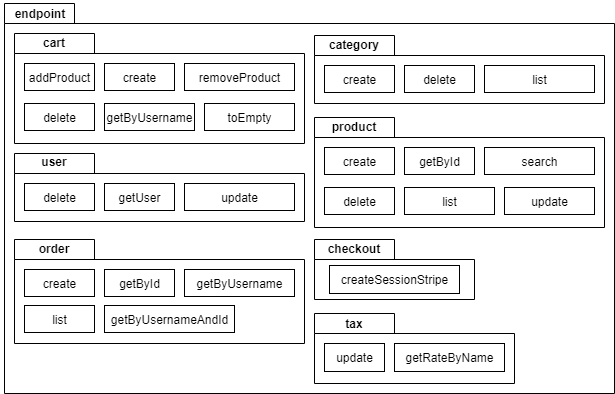
\includegraphics[scale=0.65]{res/Architettura/Backend/img/handler_package}\\
\caption{Back-end\textsubscript{G} Handler layer package diagram}
\end{figure}

Through this sequence diagram, we will show how a request can be fulfilled by all the layers. In this example, we represent the process of obtaining the details of a product and sending them to the front-end\textsubscript{G}.

\begin{figure}[H]
\centering
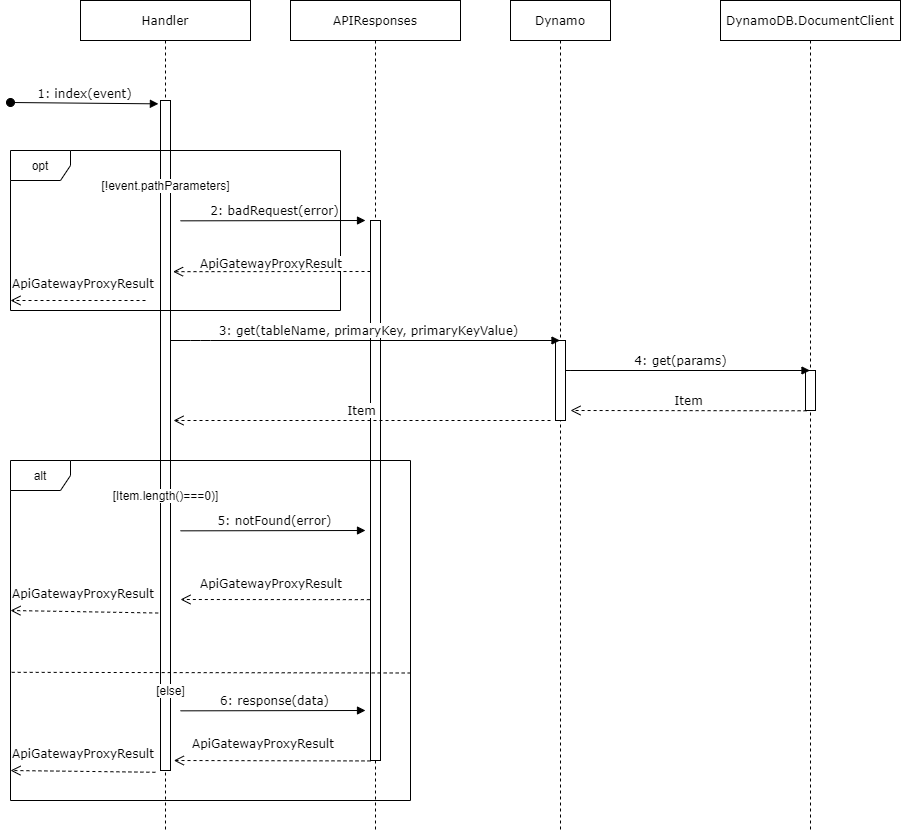
\includegraphics[scale=0.45]{res/Architettura/Backend/img/diagrammaSequenzaRicezioneProdotto}\\
\caption{Back-end\textsubscript{G} sequence diagram: obtaining product details}
\end{figure}

\begin{itemize}
\item \textbf{ApiGatewayProxyHandler} is how the function is called inside the \textit{getById} file, inside the \textit{product} domain;
\item \textbf{APIResponses} is a class inside the \textit{lib} package and manages the response to the front-end\textsubscript{G};
\item \textbf{Dynamo} is the dynamo module inside the \textit{service} module;
\item \textbf{DynamoDB.DocumentClient} is a class of the \textit{AWS-sdk} library that represents the effective database.

\end{itemize}







